\chapter*{Capitolo 3}
\addcontentsline{toc}{chapter}{Capitolo 3}

\section*{Differenza tra architetture}
\addcontentsline{toc}{section}{Differenza tra architetture}
Per capire come gli attacchi alla memoria funzionino su diverse architetture dobbiamo prima analizzare la parte fondamentale che è alla base della produzione di linguaggio macchina.\\
Nelle sezioni seguenti vedremo la differenza tra le due architetture nei registri, nello stack e nella semantica di esecuzione.
\subsection*{Architettura X86-64}
\addcontentsline{toc}{subsection}{Architettura X86-64}
Di seguito è presente una tabella per facilitare la lettura dei registri. Verranno presentati sotto la versione 64 bit, anche se è possibile trovarne a 32 o 16 bit ma con la stessa semantica.
\vspace{1cm}
\begin{center}
\begin{tabular}{| c | c c|} 
 \hline
 \textbf{Register} & \textbf{Purpose} & \textbf{Saved across calls} \\ [0.5ex] 
 \hline\hline
 \%rax & temp register; return value & No \\ 
 \hline
 \%rbx & callee-saved  & Yes \\ 
 \hline
 \%rcx & used to pass 4th argument to functions & No \\ 
 \hline
 \%rdx & used to pass 3rd argument to functions & No \\ 
 \hline
 \%rsp & stack pointer & Yes \\ 
 \hline
 \%rbp & callee-saved; base pointer & Yes \\ 
 \hline
 \%rsi & used to pass 2nd argument to functions & No \\ 
 \hline
 \%rdi & used to pass 1st argument to functions & No \\ 
 \hline
 \%r10-r11 & temporary & No \\ 
 \hline
 \%r12-r15 & callee-saved register & Yes \\ 
 \hline
\end{tabular} 
\end{center}
\vspace{1cm}
In questa architettura, come in RISC-V, i registri possono essere mantenuti in memoria o ripristinati ad ogni function call. Se ad esempio un programma ritorna da una funzione, alcuni registri come i registri temporanei oppure i registri argomento, vengono ripristinati a fine della funzione, evitando così che possano essere trovati ``sporchi" all'utilizzo successivo che ne verrà fatto.\\
Immaginiamo infatti che venga fatta una system call usando \textit{exit()}, che prende come argomento il valore contenuto nel registro \textit{rdi}. In questo caso, se il registro non venisse ripristinato e il programmatore non passasse alcun valore alla system call, il programma eseguirebbe quello che era stato precedentemente salvato nel nel registro \textit{rdi}, che quindi cambierebbe valore in base a come è stato eseguito il programma. Avremmo quindi un comportamento inatteso dovuto al fatto che il compilatore non si impegna a ripristinare i registri una volta che vengono utilizzati.\\
Un altro esempio di registro ripristinato è \textit{rax} che dovendo fornire l'indirizzo di ritorno della funzione deve per forza essere sovrascritto ad ogni esecuzione.
I registri \textit{calle-saved} sono invece salvati dal chiamante (chi chiama la funzione) e sono registri tipicamente \textit{general purpose} che vengono utilizzati in casi specifici.\\
\newline
Di particolare interesse sono quindi i registri \textit{rax} che mantiene l'indirizzo di ritorno, \textit{rsp} che mantiene lo stack pointer, ovvero un puntatore che indica la posizione nello stack dell'istruzione eseguita in un qualunque momento a runtime e \textit{rbp} che è il base pointer dello stack, indica dove inizia e viene utilizzato per salvare \textit{rsp} durante le chiamate a funzione e ripristinato con un semplice ``\textit{mov rsp, rbp}".\\
\newline
Il compilato seguente fa vedere come in x86\_64 venga gestita una semplice chiamata a funzione. In questo caso viene salvato lo stack pointer dentro il base pointer, poi caricata la stringa ``Hello World" nel registro argomento \textit{rdi} per poi chiamare tramite \textit{call} la funzione \textit{printf()} definita nella GOT. Continuando poi viene settato 0 come valore di ritorno e viene fatta la \textit{pop} del registro \textit{rbp} per ripristinare il vecchio frame pointer. Nella istruzione \textit{ret} viene fatta la pop dell'indirizzo di ritorno dallo stack e si salta a questo indirizzo, ripristinando il controllo del flusso del programma al chiamante.\\
In questa esecuzione si ha già una grande differenza con RISC-V. In questo caso infatti l'istruzione call fa il push dell'indirizzo di ritorno sullo stack e trasferisce il controllo alla funzione che viene chiamata. Su RISC-V si adotta un approccio totalmente diverso, specificando nella funzione chiamante il salvataggio dell'indirizzo di ritorno. Inoltre in RISC-V non viene utilizzato lo stack per salvare l'indirizzo di ritorno, ma l'apposito registro ra. Questo complica la vita di un attaccante, come si vedrà in seguito.
\begin{minted}[escapeinside=||,mathescape=true]{c}
0x0000000000001149 <+0>:     endbr64
0x000000000000114d <+4>:     push   %rbp
0x000000000000114e <+5>:     mov    %rsp,%rbp
0x0000000000001151 <+8>:     lea    0xeac(%rip),%rax        |# 0x2004|
0x0000000000001158 <+15>:    mov    %rax,%rdi
0x000000000000115b <+18>:    mov    $0x0,%eax
0x0000000000001160 <+23>:    call   0x1050 |<printf@plt>|
0x0000000000001165 <+28>:    mov    $0x0,%eax
0x000000000000116a <+33>:    pop    %rbp
0x000000000000116b <+34>:    ret   
\end{minted}
\subsection*{Architettura RISC-V}
Di seguito è presente una tabella per mostrare la struttura dei registri implementati dell'ISA RISC-V, tutti a 32 bit.
\addcontentsline{toc}{subsection}{Architettura RISC-V}
\vspace{1cm}
\FloatBarrier
\begin{figure}[!htbp]
    \centering
    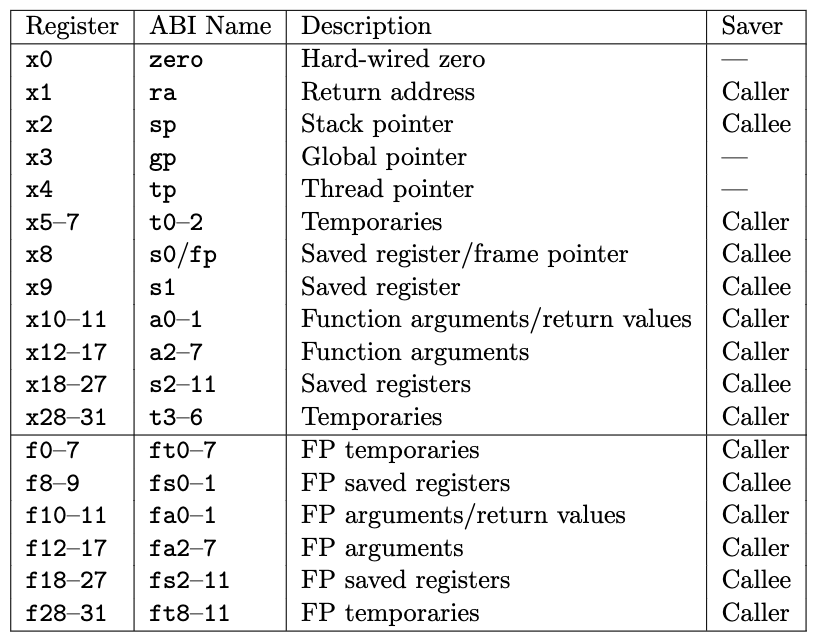
\includegraphics[width=0.7\linewidth]{images/riscv-registers.png}
\end{figure}
\FloatBarrier
\vspace{1cm}
Analogamente a quanto visto per l'altra architettura, anche in questa sono presenti alcuni registri che sono conservati tra chiamata di funzione e altri invece che vengono ripristinati.\\
Tra i registri essenziali sottolineiamo \textit{ra} che contiene il return address, come il registro \textit{rax}, \textit{sp} che sarà lo stack pointer, analogamente a \textit{rsp} e \textit{a0-a7} saranno registri dedicati agli argomenti delle funzioni. Anche in questa ISA i registri argomento, lo stack pointer e l'indirizzo di ritorno vengono ripristinati, mente altri registri chiamati ``registri s" o ``saved registers" vengono gestiti dal chiamante. s0 è invece il frame pointer.\\
\newline
Tipicamente in RISC-V tutti i registri tranne \textit{x0} (collegato al valore 0) sono general purpose e possono essere utilizzati per fare molteplici operazioni, sta al programmatore, in caso di scrittura del programma in codice macchina, oppure al compilatore di utilizzarli secondo le calling conventions \cite{RISCV}.\\
\newline
Nel seguente compilato, analizziamo le istruzioni utilizzate e la differenza con architettura tradizionale.\\
Per prima cosa si può notare che inizialmente viene decrementato lo stack pointer di 16 byte per far spazio alle istruzioni successive, poi viene salvato l'indirizzo di ritorno 8 byte sopra lo stack pointer per essere ripristinato in seguito. 
S0 (il frame pointer) viene poi salvato sullo stack e viene caricata la stringa ``Hello World" sul registro argomento a0. Viene poi fatta una \textit{jal} (jump and link) all'indirizzo della \textit{printf()}, salvando nel registro ra l'indirizzo di ritorno della funzione. Su a0 si salverà il valore di ritorno della funzione, in questo caso 0 e si ripristineranno i vecchi registri, compreso il frame pointer. All'istruzione \textit{ret} si ritornerà dalla funzione all'indirizzo contenuto dentro il registro \textit{ra}.  
\begin{minted}[escapeinside=||,mathescape=true]{c}
0x0000000000000668 <+0>:     addi    sp,sp,-16
0x000000000000066a <+2>:     sd      ra,8(sp)
0x000000000000066c <+4>:     sd      s0,0(sp)
0x000000000000066e <+6>:     addi    s0,sp,16
0x0000000000000670 <+8>:     auipc   a0,0x0
0x0000000000000674 <+12>:    addi    a0,a0,32 |# 0x690|
0x0000000000000678 <+16>:    jal     ra,0x5a0 |<printf@plt>|
0x000000000000067c <+20>:    li      a5,0
0x000000000000067e <+22>:    mv      a0,a5
0x0000000000000680 <+24>:    ld      ra,8(sp)
0x0000000000000682 <+26>:    ld      s0,0(sp)
0x0000000000000684 <+28>:    addi    sp,sp,16
0x0000000000000686 <+30>:    ret
\end{minted}
\section*{Prologo ed Epilogo delle funzioni}
\addcontentsline{toc}{section}{Prologo ed Epilogo delle funzioni}
Nello stack, per gestire le funzioni, il compilatore pone dei pezzi di codici per gestire lo stato dei registri, caricare valori e ripristinarli. Queste sezioni vengono chiamate prologo (all'inizio) ed epilogo (alla fine) di ogni funzione.\\
Nelle due architetture prologhi ed epiloghi differiscono perché lo stack (e i registri) vengono gestiti in modo diverso. È fondamentale capire la differenza per gestire poi gli attacchi, che dovranno sempre fare riferimento a queste sezioni per poter funzionare. Prologhi ed epiloghi possono venire usati attivamente come gadget per ``costruire" funzioni arbitrarie. Il seguente prologo su architettura x86 fa il push del base pointer sullo stack, salva il base pointer e sottrae N allo stack pointer per fare spazio ad eventuali variabili / buffer nello stack.
\begin{minted}[escapeinside=||,mathescape=true]{c}
push       ebp
mov	ebp, esp
sub	esp N 
\end{minted}
L'epilogo in queta architettura ripristina lo stack pointer, facendo l'operazione opposta a quanto era stato fatto precedentemente nell'epilogo, toglie ebp dallo stack e fa la return. Ci possono essere più modi per fare prologo ed epilogo, che dipendono principalmente dal flavour dell'architettura e dal tipo di compilatore ed ottimizzazione che il programmatore sta usando.
\begin{minted}[escapeinside=||,mathescape=true]{c}
mov	esp, ebp
pop	ebp
ret
\end{minted}
Su una architettura x86, in una ottica di ROP, ci aspettiamo quindi di trovare un grande numero di gadget contenenti le istruzioni \textit{mov ebp, esp} e \textit{mov ebp, esp}, anche se è sempre più facile costruire un epilogo durante una chain di gadget perché le istruzioni di epilogo sono più vicine all'istruzione ret e quindi utilizzabili senza compromettere la stabilità del programma.\\
\newline
In RISC-V prologo ed epilogo si svologno in modalità diverse, questo per vari motivi legati all'architettura. Dalle calling convention di RISC-V \cite{Arrvindh} si sottolinea che.
\begin{itemize}
    \item Il registro SP deve avere lo stesso valore sia all'entrata che all'uscita della funzione, a meno che il valore dell'indirizzo di ritorno venga salvato sullo stack
    \item Tutti i registri s devono avere lo stesso valore sia all'entrata che all'uscita della funzione
    \item La funzione deve ritornare al valore contenuto in ra, in condizioni di normale esecuzione.
\end{itemize}
Durante l'epilogo avviene la ``save sequence" in cui si salva l'indirizzo di ritorno sullo stack e si decrementa \textit{sp} in base a quanto spazio deve essere conservato nello stack per salvare i dati futuri. In questo caso si decrementa di 16 byte perché l'unico dato da salvare (di 8 byte) è \textit{ra}.
\begin{minted}[escapeinside=||,mathescape=true]{c}
addi sp ,sp , -16
sd ra ,8(sp)
\end{minted}
Avviene poi la ``restore sequence" in cui si carica (load) in ra l'indirizzo di ritorno precedentemente salvato, e si ripristina lo stack pointer per far continuare il flusso del programma. È importante sottolineare che i registri argomento, che in RISC-V sono di più rispetto a x86\_64, quando sono utilizzati devono essere tutti ripristinati a 0. Nelle calling conventions si specifica che in caso si utilizzino i registri t (temporanei) devono essere usati solamente prima delle chiamate a funzione.
\begin{minted}[escapeinside=||,mathescape=true]{c}
mv a0 , zero
mv a1 , zero
ld ra ,8(sp)
addi sp ,sp ,16
ret
\end{minted}
\section*{Leaf Functions}
\addcontentsline{toc}{section}{Leaf Functions}
Le \textit{Leaf Function} o ``callee", sono funzioni che nella programmazione tradizionale vengono chiamate da un ``caller" (chiamante). La funzione \textit{main()} è una funzione ``caller" perché fa partire tutte le altre funzioni, ma è anche una ``callee" perche di fatto viene chiamata dalla libc tramite la direttiva ``\_\_libc\_start\_main" che fa partire il programma. In generale le funzioni chiamate eseguono un task e restituiscono il risultato alla funzione chiamante, terminando con un certo codice di uscita.\\
\newline
In RISC-V è importante analizzare questo tipo di funzioni perché non è possibile utilizzare una leaf function per eseguire una ROP, ma è possibile utilizzare solo epiloghi di funzioni non leaf.\\
Questo è causato dal fatto che le funzioni leaf terminano con una return (per restituire il risultato al chiamante) invece che con una \textit{jump and link} che utilizza il registro \textit{ra} per salvare l'indirizzo di ritorno. L'attaccante che vuole sovrascrivere \textit{ra} dovrà per forza passare da una funzione non leaf per avere un entrypoint d'attacco o un gadget che permette di andare avanti nella chain di gadget.\\
In figura \ref{ref:leaf-non-leaf} si può vedere come differiscono le funzioni leaf da quelle non leaf. Una funzione non leaf (ad esempio il \textit{main()}) è una funzione che chiama altre funzioni, e quindi a livello di disassemblato non termina con una \textit{ret}. Le funzioni leaf invece sono funzioni (di solito molto semplici) che non utilizzano altre funzioni ed eseguono semplicemente l'operazione richiesta.
\vspace{1cm}
\FloatBarrier
\begin{figure}[!htbp]
    \centering
    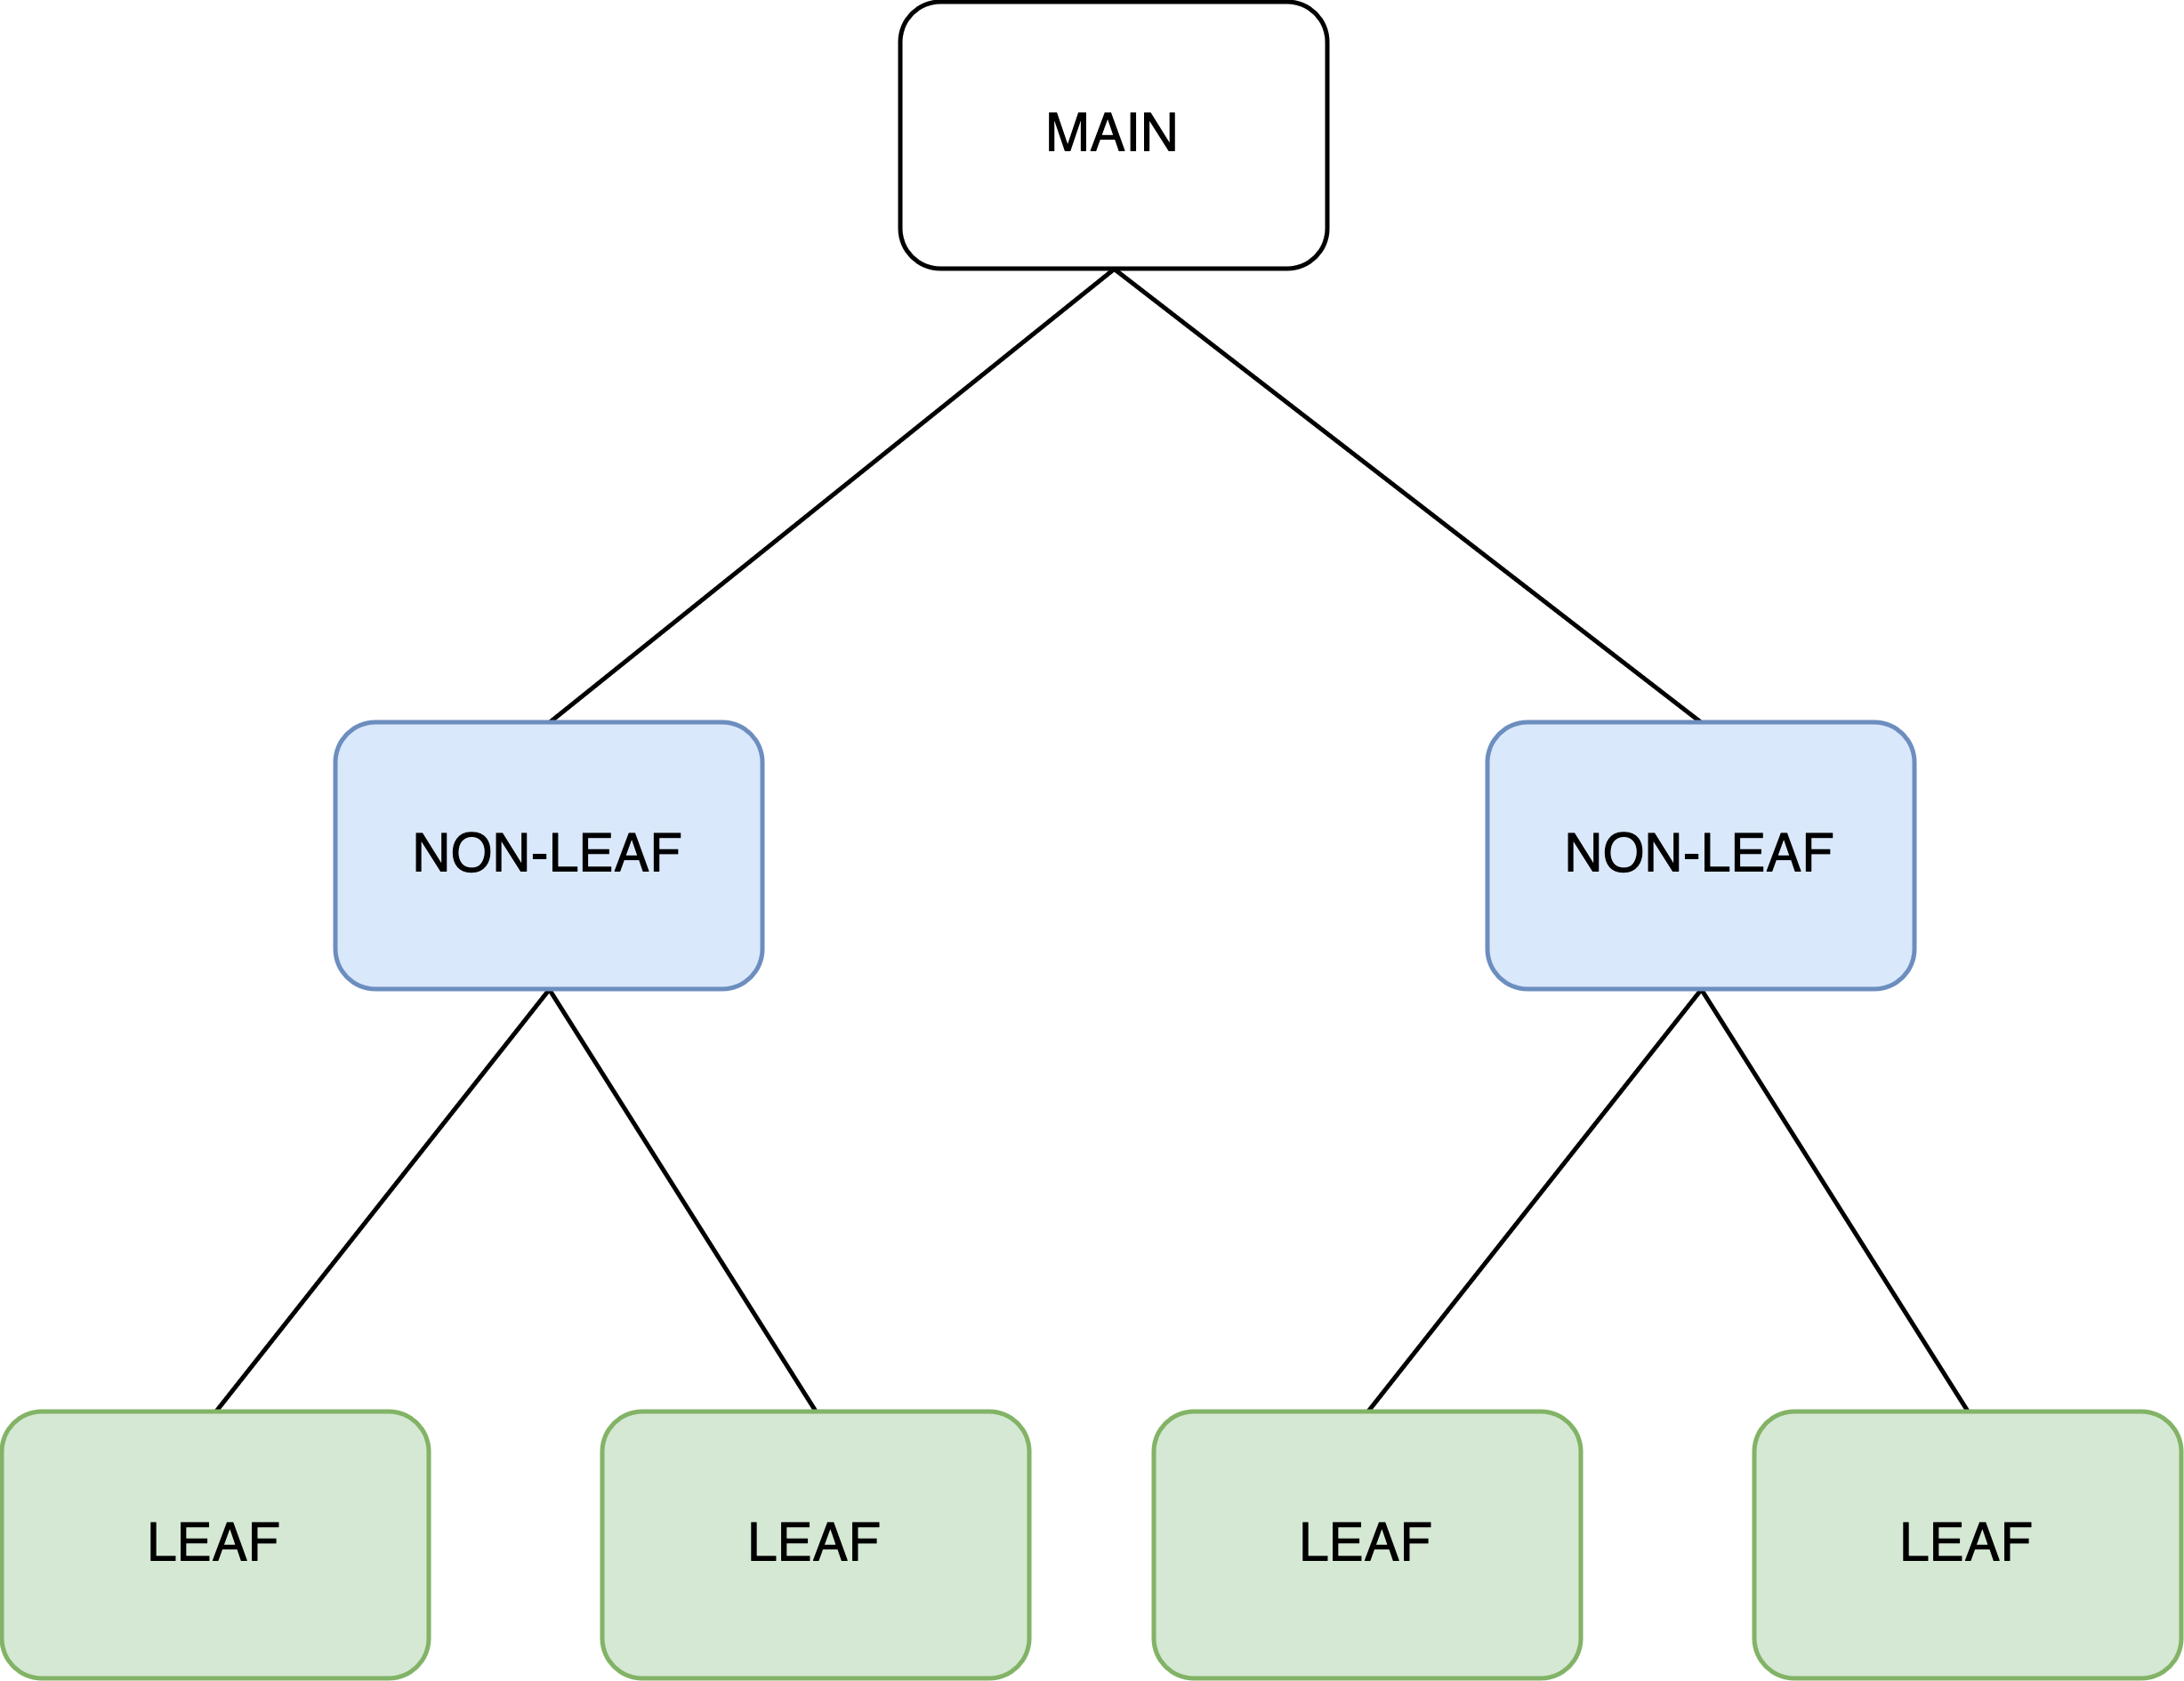
\includegraphics[width=0.6\linewidth]{images/leaf-functions.png}
    \caption{Leaf e Non-Leaf functions}
    \label{ref:leaf-non-leaf}
\end{figure}
\FloatBarrier
\vspace{1cm}
Questa è una prima grande limitazione nel panorama di ROP su RISC-V, dato che il numero possibile di gadget che riguardano gli epiloghi di funzione è ristretto ora solo a questo tipo di funzioni chiamanti. A parità di istruzioni, mentre su x86\_64 è possibile utilizzare solo lo stack per gestire l'indirizzo di ritorno, nel caso di RISC-V il registro ra è limitante e deve essere opportunatamente manipolato nelle non leaf function per avere un attacco efficace. In architetture x86\_64 il problema di leaf functions non si pone perché l'indirizzo di ritorno è sempre gestito sullo stack e una istruzione che sia \textit{jmp} o \textit{ret} farà sempre riferimento a quello.\\
La seguente funzione è una leaf function che dichiara una variabile intera, la mette uguale a 1 e poi fa la return. Si può vedere che nell'epilogo della funzione è impossibile manipolare \textit{ra} e di conseguenza l'indirizzo di ritorno perché non è presente, ma è possibile fare solo una \textit{ret}. Se si atterrasse tramite overflow a un qualunque indirizzo di questa funzione il programma andrebbe in crash o non subirebbe un exploit funzionante.\\
\begin{minted}[escapeinside=||,mathescape=true]{c}
0x0000000000000668 <+0>:     addi    sp,sp,-32
0x000000000000066a <+2>:     sd      s0,24(sp)
0x000000000000066c <+4>:     addi    s0,sp,32
0x000000000000066e <+6>:     li      a5,1
0x0000000000000670 <+8>:     sw      a5,-20(s0)
0x0000000000000674 <+12>:    nop
0x0000000000000676 <+14>:    ld      s0,24(sp)
0x0000000000000678 <+16>:    addi    sp,sp,32
0x000000000000067a <+18>:    ret
\end{minted} 
In x86\_64 indipendentemente dal tipo di funzione è invece possibile fare un jump e manipolare i successivi indirizzi di ritorno salvati nello stack. Nel codice seguente, si ha la stessa leaf function del programma compilato per RISC-V. Qua è evidente che è possibile manipolare comunque l'indirizzo di ritorno perché il prologo e l'epilogo della funzione lavorano sullo stack e base pointer.
\begin{minted}[escapeinside=||,mathescape=true]{c}
0x0000000000001149 <+0>:     endbr64
0x000000000000114d <+4>:     push   %rbp
0x000000000000114e <+5>:     mov    %rsp,%rbp
0x0000000000001151 <+8>:     movl   $0x1,-0x4(%rbp)
0x0000000000001158 <+15>:    nop
0x0000000000001159 <+16>:    pop    %rbp
0x000000000000115a <+17>:    ret
\end{minted} 

Si sottolinea dato che il programma è stato compilato con tutte le mitigazioni possibili di sicurezza, è presente l'istruzione \textit{endbr64} (end branch) utilizzata per evitare salti indesiderati tra funzioni. 
\section*{Differenze tra ROP su RISC-V e x86\_64}
\addcontentsline{toc}{section}{Differenze tra ROP su RISC-V e x86\_64}
Nonostante è stato dimostrato che sfruttando un overflow ed una \textit{libc()} all'interno di un programma RISC-V è possibile avere un linguaggio turing completo tramite ROP, il numero di istruzioni per gadget su questa architettura è generalmente maggiore. Si analizza in primo luogo il gadget minimo che serve per fare un salto (gadget NOP) \cite{arxivRISCVROP}.
\begin{minted}[escapeinside=||,mathescape=true]{c}
c.ldsp ra, 8(sp)
c.addi sp, 0x0
c.jr ra
\end{minted} 
È possibile paragonare questa serie di istruzioni ad una semplice \textit{ret} di 1 byte su architettura x86\_64. In uno scenario in cui l'overflow da inserire è limitato, è meno probabile quindi riuscire ad eseguire una ROP su RISC-V rispetto a x86. Avere un numero maggiore di istruzioni per gadget causa delle complicazioni. Analizzando il codice assembly seguente
\begin{minted}[escapeinside=||,mathescape=true]{c}
c.ldsp ra, 0x28(sp)
c.ldsp s0, 0x20(sp)
c.ldsp a0, 0(sp)
c.ldsp a1, 8(sp)
c.ldsp s1, 0x18(sp)
c.ldsp s2, 0x10(sp)
c.addi16sp sp, 0x30
c.jr ra
\end{minted} 
Si può notare che se un attaccante vuole usare le istruzioni ``basse", ovvero vicino a \textit{c.jr ra}, non può sempre saltare direttamente all'istruzione voluta. Questo perché se ad esempio il salto avvenisse a \textit{c.ldsp s2, 0x10(sp)}, con la volontà di preservare i registri \textit{a0 a1} e \textit{s1}, il programma andrebbe in loop o in crash avendo saltato l'istruzione \textit{c.ldsp ra, 0x28(sp)} utilizzata per salvare l'indirizzo di ritorno. Questo porta due grandi limitazioni rispetto a x86\_64
\begin{itemize}
    \item Non sempre è possibile trovare le istruzioni che servono poste in modo contiguo
    \item L'attaccante deve focalizzarsi maggiormente su salti in prossimità dell'epilogo della funzione
\end{itemize}
Un modo di arginare almeno una parte del problema, è utilizzare dei registri che non vengono ripristinati dalla funzione, per costruire step by step un valore utile contenuto in un determinato registro. Per fare questo si utilizzano i \textit{callee-saved} registers, come i registri S. Si evitano invece i registri A (argomento) perché è altamente probabile, soprattutto per quelli bassi come \textit{a0}, \textit{a1} e \textit{a2} che vengano utilizzati dal compilatore come registri argomento della funzione.\\
Vediamo un esempio di chain di gadget in una ROP usando i registri S. Lo scopo della chain è quello di caricare in \textit{a0} il valore 3, invece che il valore 1 originario della funzione. Il primo gadget imposta \textit{s1} a 1 
\begin{minted}[escapeinside=||,mathescape=true]{c}
c.ldsp ra, 8(sp)
...
c.li s1, 0x01
c.jr ra
\end{minted} 
Il secondo gadget manipola il registro \textit{a0} e \textit{s0} ma in questo momento non è importante per la chain e nell'epilogo aggiunge 1 al registro \textit{s1}.
\begin{minted}[escapeinside=||,mathescape=true]{c}
c.ldsp ra, 8(sp)
...
c.ldsp a0, 0(sp)
c.addi s0, 0x01
c.addi s1, 0x01
c.jr ra
\end{minted} 
Alla fine viene nuovamente aggiunto 1 al registro \textit{s1} che viene incrementato fino ad arrivare al valore 3. Viene poi copiato il suo contenuto dentro \textit{a0} che verrà utilizzato per fare una chiamata di funzione con l'argomento intero a 3 invece che impostato a 1.
\begin{minted}[escapeinside=||,mathescape=true]{c}
c.ldsp ra, 8(sp)
...
c.addi s1, 0x01
mv a0 s2
...
jal ra, <funzione>
c.jr ra
\end{minted} 

\section*{Esempio di ROP su RISC-V}
\addcontentsline{toc}{section}{Esempio di ROP su RISC-V}
Per capire la differenza tra attacchi ROP sulle due architetture diverse, partiamo da un esempio di ROP su architettura RISC-V. In figura \ref{ref:riscv-rop} è possibile vedere il flusso di esecuzione di un attacco che sfrutta la funzione \textit{strcpy()} come entrypoint per scrivere nello stack e sovrascrivere l'indirizzo di ritorno. In questo scenario l'ALSR, la stack protection e i canarini devono essere disabilitati affinché l'attacco funzioni.\\
\newline
Lo scopo dell'exploit è chiamare la funzione \textit{system()} con al suo interno nei registri argomento a0 e a1 i parametri necessari per aprire una shell, ovvero con \textit{a0 = /bin/sh} e \textit{a1 = 0}.\\
Sovrascrivendo l'indirizzo di ritorno grazie all'overflow è possibile atterrare sul primo gadget che setta a 0 i registri. Verrà poi utilizzato un secondo gadget per caricare nel registro a7 il valore 221, ovvero la system call numero 221 che su sistemi RISC-V è la \textit{execve()}. Alla fine viene copiato nel registro a0 quello che si trova nello stack (che ora è manipolato dall'attaccante che immetterà l'overflow e la stringa \textit{/bin/sh}).\\
A fine attacco viene fatta la ecall che di fatto eseguirà il seguente codice ricostruito tramite ROP.
\begin{minted}[escapeinside=||,mathescape=true]{c}
execve("/bin/sh", 0)
\end{minted} 
Questa tecnica è anche chiamata ``code reuse".\\
\newline
Un attaccante che ha accesso al sistema può scegliere l'approccio ROP anche per avere una persistent backdoor, compilando un progamma e lasciando per tutto lo stack delle funzioni e quindi dei gadget per ricostruire una chain all'occorrenza. Questo è un modo per bypassare i comuni antivirus che basano la detection su delle ``signature" del codice, o che fanno solo analisi statica del programma.\\
In questo scenario, come tutte le ROP, anche se il programma è compilato con DEP (data execution prevention) e con le mitigazioni dello stack, l'exploit avrà comunque successo perché non viene immesso alcuno shellcode, ma solo dati utili a costruire la chain e la stringa \textit{/bin/sh}.
\vspace{1cm}
\FloatBarrier
\begin{figure}[!htbp]
    \centering
    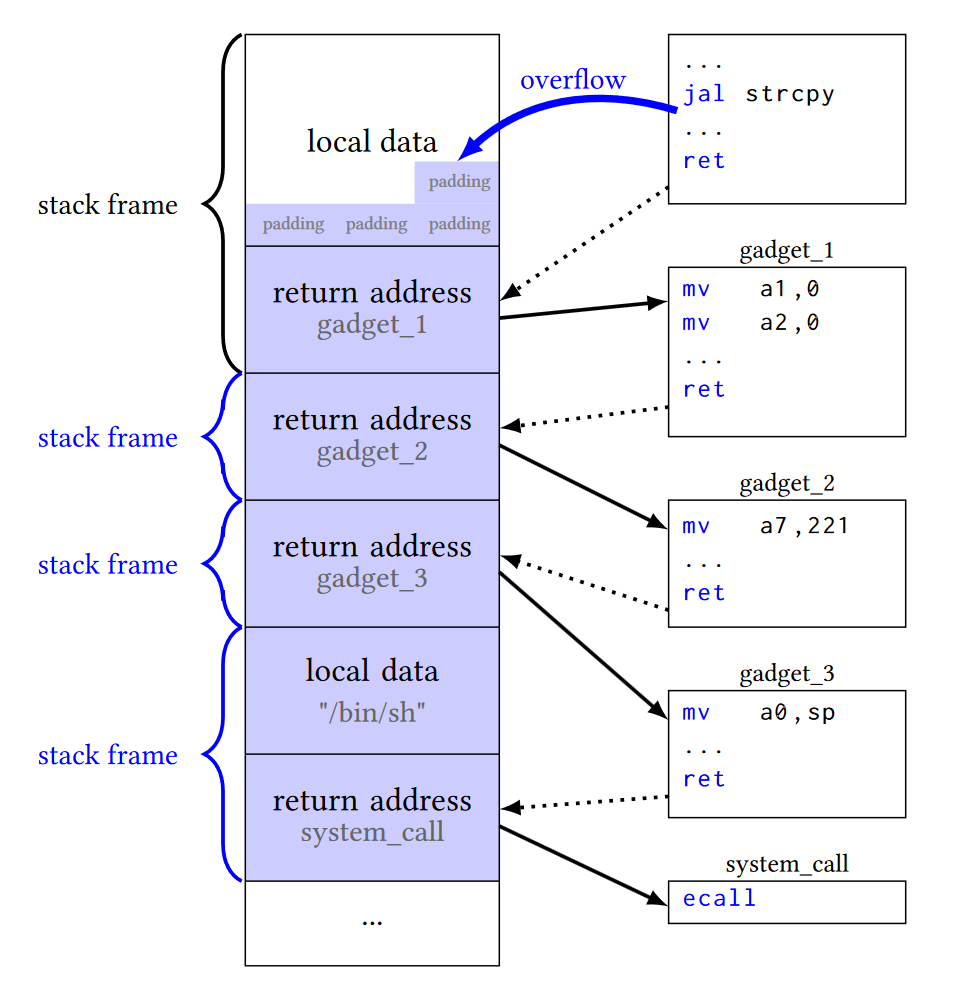
\includegraphics[width=0.8\linewidth]{images/riscv-rop.png}
    \caption{Logica di un attacco ROP su RISC-V}
    \label{ref:riscv-rop}
\end{figure}
\FloatBarrier
\vspace{1cm}
Se questa ROP viene compilata con librerie dinamiche, è probabile trovare l'istruzione ``ecall" mancante. Questo perché si utilizzano funzioni di libreria che fanno da wrapper, come nel caso della \textit{system()}. Se il programma fosse compilato con questo approccio, al posto dell'ultimo gadget ci sarebbe stata una \textit{jal} alla funzione \textit{system()} della libc. Questo avrebbe potuto causare dei problemi dato che a tutti gli effetti viene poi chiamata una funzione che ha un prologo ed un epilogo e quindi i registri verranno manipolati causando un potenziale crash del programma. L'attaccante avrebbe dovuto quindi analizzare dentro la funzione \textit{system()} dove viene eseguita la system call e saltare direttamente a quell'indirizzo.

\section*{Esempio di ROP su x86}
\addcontentsline{toc}{section}{Esempio di ROP su x86}
Su questa architettura come detto in precedenza lo stack non fa riferimento a dei registri per contenere l'indirizzo di ritorno, ma lo memorizza direttamente lui stesso.\\
Nel seguente attacco in figura \ref{ref:x86-rop} si può vedere che dopo l'overflow, quando la funzione farà l'istruzione \textit{ret}, l'attaccante sarà in grado di saltare all'indirizzo puntato da \textit{esp} in seguito a \textit{pop \%edx}. In questo caso \textit{esp} punterà al'indirizzo arbitrario scelto dall'attaccante (\textit{0xdeadbeef}), messo nello stack, che sarà l'indirizzo del prossimo gadget. In questo modo è possibile creare catene di gadget utilizzando solamente byte immessi nello stack dall'attaccante.
\vspace{1cm}
\FloatBarrier
\begin{figure}[!htbp]
    \centering
    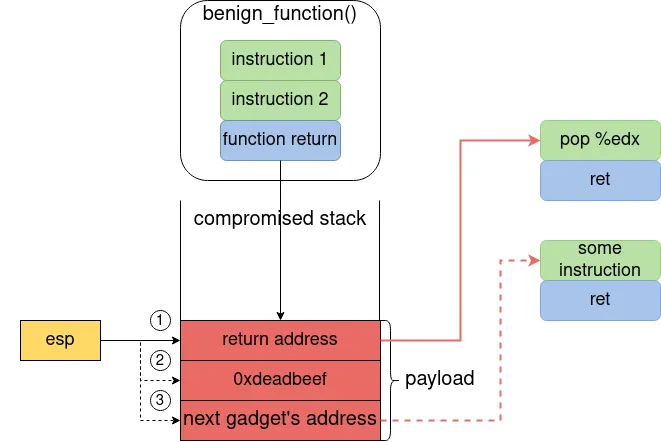
\includegraphics[width=0.7\linewidth]{images/x86-rop.png}
    \caption{Logica di un attacco ROP su x86} \cite{infosecwriteupsROP}
    \label{ref:x86-rop}
\end{figure}
\FloatBarrier
\vspace{1cm}
Riassumendo, possiamo dire che l'architettura RISC-V è basata su \textit{load e store} nei registri, mentre quella x86 e x86\_64 è completamente stack based e si basa su istruzioni come \textit{POP e RET}. In quest'ultima architettura viene infatti usata la \textit{POP} per prendere i valori dell'indirizzo a cui saltare sullo stack e la \textit{RET} per saltare a quell'indirizzo. Il fatto che esista una singola istruzione permette all'attaccante di utilizzare qualunque epilogo di funzione per costruire una ROP-chain. Su RISC-V non è possibile seguire questa metodologia.\\
\section*{Costruzione della ROP-chain e gadget essenziali}
\addcontentsline{toc}{section}{Costruzione della ROP-chain e gadget essenziali}
Per costruire una chain, qui è infatti necessario ripristinare lo stato dei registri che si sono usati. Come si può vedere nell'esempio seguente al fine di utilizzare questo gadget per caricare nel registro \textit{s1} i valori decisi dall'attaccante, è anche necessario sfruttare un payload maggiore, dato che \textit{s0, s2, s3} devono mantenere lo stato tra le chiamate a funzione, come definito nella calling convention. Perciò l'attaccante deve fornire dei valori fasulli per far sì che questi registri siano effettivamente caricati dallo stack.
\begin{minted}[escapeinside=||,mathescape=true]{c}
li    a0, 0
ld    ra, 40(sp)
ld    s0, 32(sp)
ld    s1, 24(sp)
ld    s2, 16(sp)
ld    s3, 8(sp)
addi  sp, sp, 48
ret
\end{minted}
Una delle path di attacco per una ROP su RISC-V è quindi la seguente
\begin{enumerate}
    \item Provocare un overflow in memoria (stack o heap)
    \item Individuare una funzione (di solito nella libc) che manipola i registri necessari (a0-a7 / s2-s11)
    \item Caricare nel registro \textit{ra} l'indirizzo di ritorno al prossimo gadget
    \item Riempiere lo stack di valori necessari per sovrascrivere i registri interessati
    \item Ripetere il punto 2 finché non si è costruito il codice arbitrario
\end{enumerate}
Di solito il primo gadget che si cerca è sempre un gadget che carica il maggior numero di registri possibili, in modo che l'attaccante abbia il payload ``già caricato" di alcuni registri. Il seguente gadget è preziosissimo, perché permette di caricare di un valore arbitrario passato sullo stack i registri a0-a7, ovvero i registri argomento usati dall'architettura. Riuscendo a manipolare questi registri sarà infatti possibile eseguire una system call con fino a 7 argomenti.\\
Questo è anche un gadget ``chainable" perché parte di una non-leaf function e ciò permette di decidere anche il prossimo indirizzo di ritorno caricando un valore a \textit{72(sp)}.
\begin{minted}[escapeinside=||,mathescape=true]{c}
ld	ra,72(sp)
ld	a0,8(sp)
ld	a1,16(sp)
ld	a2,24(sp)
ld	a3,32(sp)
ld	a4,40(sp)
ld	a5,48(sp)
ld	a6,56(sp)
ld	a7,64(sp)
ld	s1,80(sp)
addi      sp,sp,88
jr	ra
\end{minted}
Altri gadget preziosi sono quelli che permettono di eseguire system call. Il seguente gadget imposterà 1 come argomento della system call \textit{exit}, caricherà il registro \textit{a7} del valore corrispondente al numero della systemcall e alla fine chiamerà la system call.
\begin{minted}[escapeinside=||,mathescape=true]{c}
li a0, 1
li a7, 93
ecall
\end{minted}
Altri gadget essenziali, sono quelli che permettono di saltare a determinati registri, valori o che permettono di eseguire calcoli nei registri, ma non verranno qua presentati.\\
Per concludere, è possibile dare delle linee guida per la costruzione di una ROP su RISC-V, rispetto a una su x86\_64.
\begin{itemize}
    \item La ROP exploitation è relegata solo a epiloghi di funzioni non-leaf
    \item L'attaccante deve essere in grado di manipolare il registro ra scrivendo a multipli di 8 byte nello stack
    \item Deve essere possibile a caricare un immediato di N byte nel registro sp per ripristinare lo stack pointer
    \item Si deve trovare una sequenza di istruzioni extra per eseguire i calcoli necessari
    \item L'attacco deve finire principalmente con una return
\end{itemize}
Alla luce di questo, sviluppare un attacco ROP su RISC-V è generalmente più difficile rispetto ad un attacco ROP sull'architettura x86 e x86\_64, sia per difficoltà nella ricerca di gadget, sia per il numero di gadget disponibili.\\
È da sottolineare che x64 di solito richiede meno gadget durante un attacco ROP, per la sua struttura dei registri, ma la concatenazione dei gadget è di solito più complessa a causa dello spazio maggiore in byte che richiedono i registri essendo un architettura a 64 bit. 